    \item Consider a system of linear equations:
    \begin{align*}
        x-2y+3z &= -1, \\
        x-3y+4z &= 1, \quad \text{and} \\
        -2x+4y-6z &= k
    \end{align*}
    The value of $k$ for which the system has infinitely many solutions is \underline{\hspace{2cm}}.
    \hfill{\brak{\text{GATE EC 2015}}}
    \item The value of $p$ such that the vector $\myvec{1\\ 2\\ 3}$ is an eigenvector of the matrix $\myvec{4 & 1 & 2\\ p & 2 & 1\\ 14 & -4 & 10}$ is \underline{\hspace{2cm}}.
    \hfill{\brak{\text{GATE EC 2015}}}

    \item In the circuit shown, at resonance, the amplitude of the sinusoidal voltage \brak{in Volts} across the capacitor is \underline{\hspace{2cm}}.
    \begin{figure}[H]
        \centering
        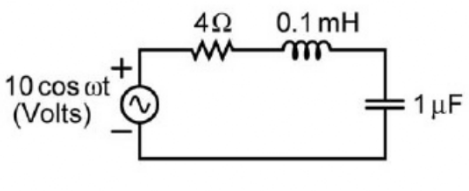
\includegraphics[width=0.4\columnwidth]{figs/q16.png}
        \caption*{}
        \label{fig:q16}
    \end{figure}
    
    \hfill{\brak{\text{GATE EC 2015}}}

    \item In the network shown in the figure, all resistors are identical with $R=300~\ohm$. The resistance $R_{ab} \brak{\text{in } \ohm}$ of the network is \underline{\hspace{2cm}}.
    \begin{figure}[H]
        \centering
        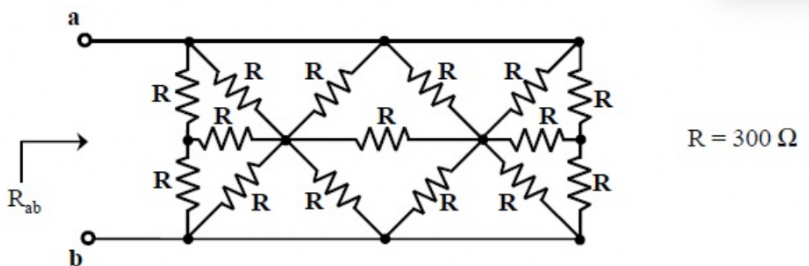
\includegraphics[width=0.6\columnwidth]{figs/q17.png}
        \caption*{}
        \label{fig:q17}
    \end{figure}
    
    \hfill{\brak{\text{GATE EC 2015}}}

    \item In the given circuit, the values of $V_{1}$ and $V_{2}$ respectively are
    \begin{figure}[H]
        \centering
        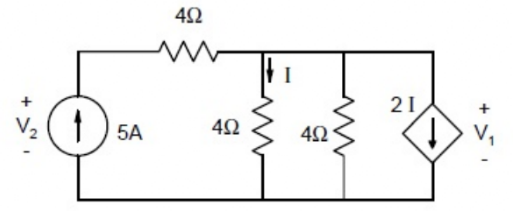
\includegraphics[width=0.5\columnwidth]{figs/q18.png}
        \caption*{}
        \label{fig:q18}
    \end{figure}
    \begin{enumerate}
        \begin{multicols}{2}
            \item 5 V, 25 V
            \item 10 V, 30 V
            \item 15 V, 35 V
            \item 0 V, 20 V
        \end{multicols}
    \end{enumerate}
    
    \hfill{\brak{\text{GATE EC 2015}}}

    \item A region of negative differential resistance is observed in the current voltage characteristics of a silicon PN junction if
    \begin{enumerate}
        \item both the P-region and the N-region are heavily doped
        \item the N-region is heavily doped compared to the P-region
        \item the P-region is heavily doped compared to the N-region
        \item an intrinsic silicon region is inserted between the P-region and the N-region
    \end{enumerate}
    
    \hfill{\brak{\text{GATE EC 2015}}}

    \item A silicon sample is uniformly doped with donor type impurities with a concentration of $10^{16}/cm^{3}$. The electron and hole mobilities in the sample are $1200~cm^{2}/V-s$ and $400~cm^{2}/V-s$ respectively. Assume complete ionization of impurities. The charge of an electron is $1.6\times10^{-19}C$. The resistivity of the sample \brak{in $\ohm$-cm} is \underline{\hspace{2cm}}.
    
    \hfill{\brak{\text{GATE EC 2015}}}

    \item For the circuit with ideal diodes shown in the figure, the shape of the output $\brak{v_{out}}$ for the given sine wave input $\brak{v_{in}}$ will be
    \begin{figure}[H]
        \centering
        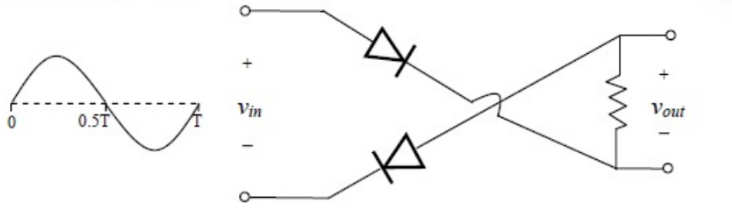
\includegraphics[width=0.5\columnwidth]{figs/q21.png}
        \caption*{}
        \label{fig:q21}
    \end{figure}
    \begin{enumerate}
        \item 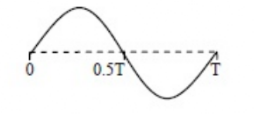
\includegraphics[width=0.4\columnwidth]{figs/q21A.png}
        \item 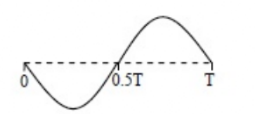
\includegraphics[width=0.4\columnwidth]{figs/q21B.png}
        \item 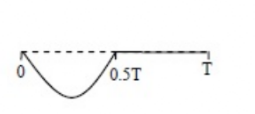
\includegraphics[width=0.4\columnwidth]{figs/q21C.png}
        \item 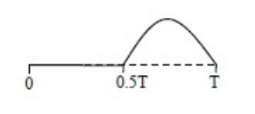
\includegraphics[width=0.4\columnwidth]{figs/q21D.png}
    \end{enumerate}
    
    \hfill{\brak{\text{GATE EC 2015}}}

    \item In the circuit shown below, the Zener diode is ideal and the Zener voltage is 6 V. The output voltage $V_{0} \brak{\text{in volts}}$ is \underline{\hspace{2cm}}.
    \begin{figure}[H]
        \centering
        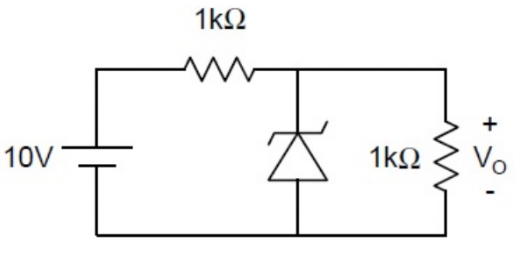
\includegraphics[width=0.4\columnwidth]{figs/q22.png}
        \caption*{}
        \label{fig:q22}
    \end{figure}
    
    \hfill{\brak{\text{GATE EC 2015}}}

    \item In the circuit shown, the switch SW is thrown from position A to position B at time $t=0$. The energy \brak{in $\mu$J} taken from the 3 V source to charge the 0.1 $\mu$F capacitor from 0 V to 3 V is
    \begin{figure}[H]
        \centering
        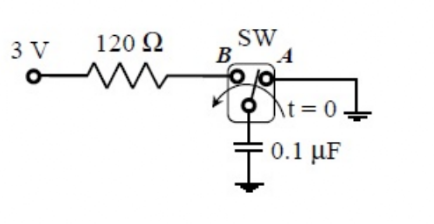
\includegraphics[width=0.5\columnwidth]{figs/q23.png}
        \caption*{}
        \label{fig:q23}
    \end{figure}
    \begin{enumerate}
        \begin{multicols}{4}
            \item 0.3
            \item 0.45
            \item 0.9
            \item 3
        \end{multicols}
    \end{enumerate}
    
    \hfill{\brak{\text{GATE EC 2015}}}

    \item In an 8085 microprocessor, the shift registers which store the result of an addition and the overflow bit are, respectively
    \begin{enumerate}
        \begin{multicols}{2}
            \item B and F
            \item A and F
            \item H and F
            \item A and C
        \end{multicols}
    \end{enumerate}
    
    \hfill{\brak{\text{GATE EC 2015}}}

    \item A 16 Kb \brak{=16,384 bit} memory array is designed as a square with an aspect ratio of one \brak{\text{number of rows is equal to the number of columns}}. The minimum number of address lines needed for the row decoder is \underline{\hspace{2cm}}.
    
    \hfill{\brak{\text{GATE EC 2015}}}

    \item Consider a four bit D to A converter. The analog value corresponding to digital signals of values 0000 and 0001 are 0 V and 0.0625 V respectively. The analog value \brak{in Volts} corresponding to the digital signal 1111 is \underline{\hspace{2cm}}.
    
    \hfill{\brak{\text{GATE EC 2015}}}

    \item The result of the convolution $x\brak{-t}*\delta\brak{-t-t_{0}}$ is
    \begin{enumerate}
        \begin{multicols}{4}
            \item $x\brak{t+t_{0}}$
            \item $x\brak{t-t_{0}}$
            \item $x\brak{-t+t_{0}}$
            \item $x\brak{-t-t_{0}}$
        \end{multicols}
    \end{enumerate}
    
    \hfill{\brak{\text{GATE EC 2015}}}

    \item The waveform of a periodic signal $x\brak{t}$ is shown in the figure.
    \begin{figure}[H]
        \centering
        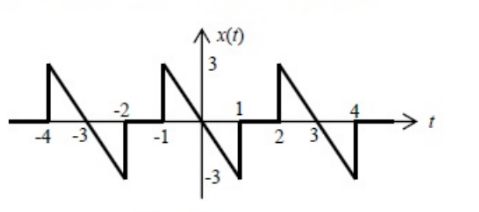
\includegraphics[width=0.5\columnwidth]{figs/q28.png}
        \caption*{}
        \label{fig:q28}
    \end{figure}
    A signal $g\brak{t}$ is defined by $g\brak{t}=x\brak{\frac{t-1}{2}}$. The average power of $g\brak{t}$ is \underline{\hspace{2cm}}.
    
    \hfill{\brak{\text{GATE EC 2015}}}

    \item Negative feedback in a closed-loop control system DOES NOT
    \begin{enumerate}
        \item reduce the overall gain
        \item reduce bandwidth
        \item improve disturbance rejection
        \item reduce sensitivity to parameter variation
    \end{enumerate}
    
    \hfill{\brak{\text{GATE EC 2015}}}

    \item A unity negative feedback system has the open-loop transfer function $G\brak{s}=\frac{K}{s\brak{s+1}\brak{s+3}}$. The value of the gain K \brak{$>0$} at which the root locus crosses the imaginary axis is \underline{\hspace{2cm}}.
    
    \hfill{\brak{\text{GATE EC 2015}}}

    \item The polar plot of the transfer function $G\brak{s}=\frac{10\brak{s+1}}{s+10}$ for $0\le\omega<\infty$ will be in the
    \begin{enumerate}
        \begin{multicols}{2}
            \item first quadrant
            \item second quadrant
            \item third quadrant
            \item fourth quadrant
        \end{multicols}
    \end{enumerate}
    
    \hfill{\brak{\text{GATE EC 2015}}}

    \item A sinusoidal signal of 2 kHz frequency is applied to a delta modulator. The sampling rate and step-size $\Delta$ of the delta modulator are 20,000 samples per second and 0.1 V, respectively. To prevent slope overload, the maximum amplitude of the sinusoidal signal \brak{in Volts} is
    \begin{enumerate}
        \begin{multicols}{2}
            \item $\frac{1}{2\pi}$
            \item $\frac{1}{\pi}$
            \item $\frac{2}{\pi}$
            \item $\pi$
        \end{multicols}
    \end{enumerate}
    
    \hfill{\brak{\text{GATE EC 2015}}}

    \item Consider the signals $s\brak{t}=m\brak{t}\cos\brak{2\pi f_{c}t}+\hat{m}\brak{t}\sin\brak{2\pi f_{c}t}$ where $\hat{m}\brak{t}$ denotes the Hilbert transform of $m\brak{t}$ and the bandwidth of $m\brak{t}$ is very small compared to $f_{c}$. The signal $s\brak{t}$ is a
    \begin{enumerate}
        \item high-pass signal
        \item low-pass signal
        \item band-pass signal
        \item double sideband suppressed carrier signal
    \end{enumerate}
    
    \hfill{\brak{\text{GATE EC 2015}}}

    \item Consider a straight, infinitely long, current carrying conductor lying on the z-axis. Which one of the following plots \brak{in linear scale} qualitatively represents the dependence of $H_{\phi}$ on r, where $H_{\phi}$ is the magnitude of the azimuthal component of magnetic field outside the conductor and r is the radial distance from the conductor?
    \begin{enumerate}
        \item \begin{figure}[H]\centering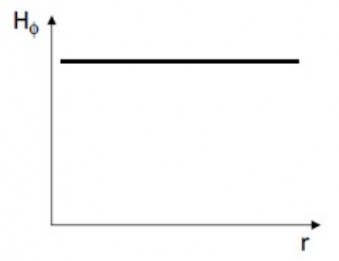
\includegraphics[width=0.4\columnwidth]{figs/q34A.png}\end{figure}
        \item \begin{figure}[H]\centering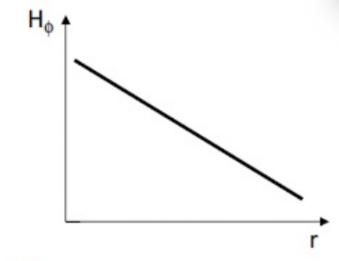
\includegraphics[width=0.4\columnwidth]{figs/q34B.png}\end{figure}
        \item \begin{figure}[H]\centering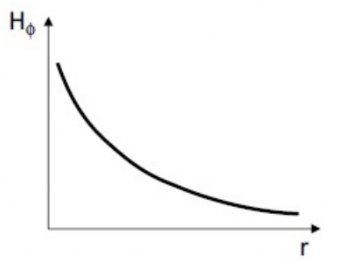
\includegraphics[width=0.4\columnwidth]{figs/q34C.png}\end{figure}
        \item \begin{figure}[H]\centering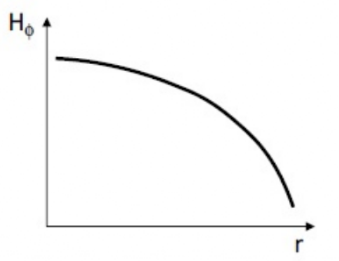
\includegraphics[width=0.4\columnwidth]{figs/q34D.png}\end{figure}
    \end{enumerate}
    
    \hfill{\brak{\text{GATE EC 2015}}}

    \item The electric field component of a plane wave traveling in a lossless dielectric medium is given by $\vec{E}\brak{z,t}=\hat{a}_{y}2 \cos\brak{10^{8}t-\frac{z}{\sqrt{2}}}V/m$. The wavelength \brak{in m} for the wave is \underline{\hspace{2cm}}.
    
    \hfill{\brak{\text{GATE EC 2015}}}

    \item The solution of the differential equation $\frac{d^{2}y}{dt^{2}}+2\frac{dy}{dt}+y=0$ with $y\brak{0}=y'\brak{0}=1$ is
    \begin{enumerate}
        \begin{multicols}{2}
            \item $\brak{2-t}e^{t}$
            \item $\brak{1+2t}e^{-t}$
            \item $\brak{2+t}e^{-t}$
            \item $\brak{1-2t}e^{t}$
        \end{multicols}
    \end{enumerate}
    
    \hfill{\brak{\text{GATE EC 2015}}}

    \item A vector $\vec{P}$ is given by $\vec{P}=x^{3}y\vec{a}_{x}-x^{2}y^{2}\vec{a}_{y}-x^{2}yz\vec{a}_{z}$. Which one of the following statements is TRUE?
    \begin{enumerate}
        \item $\vec{P}$ is solenoidal, but not irrotational
        \item $\vec{P}$ is irrotational, but not solenoidal
        \item $\vec{P}$ is neither solenoidal nor irrotational
        \item $\vec{P}$ is both solenoidal and irrotational
    \end{enumerate}
    
    \hfill{\brak{\text{GATE EC 2015}}}

    \item Which one of the following graphs describes the function $f\brak{x}=e^{-x}\brak{x^{2}+x+1}$?
    \begin{enumerate}
        \item \begin{figure}[H]\centering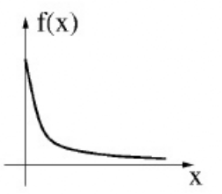
\includegraphics[width=0.4\columnwidth]{figs/q38A.png}\end{figure}
        \item \begin{figure}[H]\centering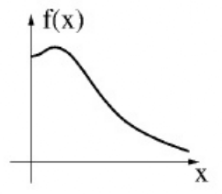
\includegraphics[width=0.4\columnwidth]{figs/q38B.png}\end{figure}
        \item \begin{figure}[H]\centering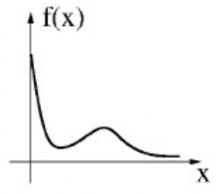
\includegraphics[width=0.4\columnwidth]{figs/q38C.png}\end{figure}
        \item \begin{figure}[H]\centering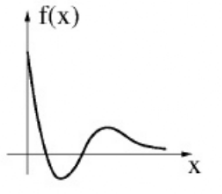
\includegraphics[width=0.4\columnwidth]{figs/q38D.png}\end{figure}
    \end{enumerate}
    
    \hfill{\brak{\text{GATE EC 2015}}}

    \item The maximum area \brak{in square units} of a rectangle whose vertices lie on the ellipse $x^{2}+4y^{2}=1$ is \underline{\hspace{2cm}}.
    
    \hfill{\brak{\text{GATE EC 2015}}}

    \item The damping ratio of a series RLC circuit can be expressed as
    \begin{enumerate}
        \begin{multicols}{2}
            \item $\frac{R^{2}C}{2L}$
            \item $\frac{2L}{R^{2}C}$
            \item $\frac{R}{2}\sqrt{\frac{C}{L}}$
            \item $\frac{2}{R}\sqrt{\frac{L}{C}}$
        \end{multicols}
    \end{enumerate}
    
    \hfill{\brak{\text{GATE EC 2015}}}

    \item In the circuit shown, switch SW is closed at $t=0$. Assuming zero initial conditions, the value of $v_{c}\brak{t}$ \brak{in Volts} at $t=1$ sec is \underline{\hspace{2cm}}.
    \begin{figure}[H]
        \centering
        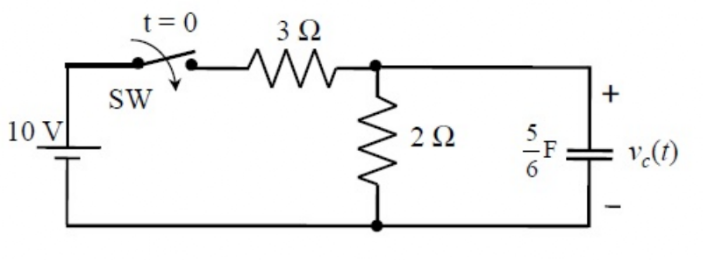
\includegraphics[width=0.5\columnwidth]{figs/q41.png}
        \caption*{}
        \label{fig:q41}
    \end{figure}
    
    \hfill{\brak{\text{GATE EC 2015}}}

    \item In the given circuit, the maximum power \brak{in Watts} that can be transferred to the load $R_{L}$ is \underline{\hspace{2cm}}.
    \begin{figure}[H]
        \centering
        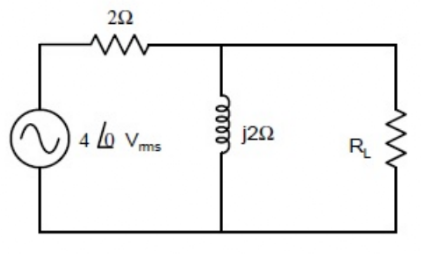
\includegraphics[width=0.5\columnwidth]{figs/q42.png}
        \caption*{}
        \label{fig:q42}
    \end{figure}
    
    \hfill{\brak{\text{GATE EC 2015}}}

    \item The built-in potential of an abrupt p-n junction is 0.75 V. If its junction capacitance \brak{$C_{J}$} at a reverse bias \brak{$V_{R}$} of 1.25 V is 5 pF, the value of $C_{J}$ \brak{in pF} when $V_{R}=7.25 V$ is \underline{\hspace{2cm}}.
    
    \hfill{\brak{\text{GATE EC 2015}}}

    \item A MOSFET in saturation has a drain current of 1 mA for $V_{DS}=0.5 V$. If the channel length modulation coefficient is 0.05 $V^{-1}$, the output resistance \brak{in k$\ohm$} of the MOSFET is \underline{\hspace{2cm}}.
    
    \hfill{\brak{\text{GATE EC 2015}}}

    \item For a silicon diode with long P and N regions, the accepter and donor impurity concentrations are $1\times10^{17}cm^{-3}$ and $1\times10^{15}cm^{-3}$ respectively. The lifetimes of electrons in P region and holes in N region are both 100 µs. The electron and hole diffusion coefficients are 49 $cm^{2}/s$ and 36 $cm^{2}/s$, respectively. Assume kT/q = 26 mV, the intrinsic carrier concentration is $1\times10^{10}cm^{-3}$ and $q=1.6\times10^{-19}C$. When a forward voltage of 208 mV is applied across the diode, the hole current density \brak{in $nA/cm^{2}$} injected from P region to N region is \underline{\hspace{2cm}}.
    
    \hfill{\brak{\text{GATE EC 2015}}}

    \item The Boolean expression $F\brak{X,Y,Z}=\overline{X}Y\overline{Z}+X\overline{Y}\overline{Z}+X Y\overline{Z}+XYZ$ converted into the canonical product of sum \brak{POS} form is
    \begin{enumerate}
        \item $\brak{X+Y+Z}\brak{X+Y+\overline{Z}}\brak{X+\overline{Y}+\overline{Z}}\brak{\overline{X}+Y+\overline{Z}}$
        \item $\brak{X+\overline{Y}+Z}\brak{\overline{X}+Y+\overline{Z}}\brak{\overline{X}+\overline{Y}+Z}\brak{\overline{X}+\overline{Y}+\overline{Z}}$
        \item $\brak{X+Y+Z}\brak{\overline{X}+Y+\overline{Z}}\brak{X+\overline{Y}+Z}\brak{\overline{X}+\overline{Y}+\overline{Z}}$
        \item $\brak{X+\overline{Y}+\overline{Z}}\brak{\overline{X}+Y+Z}\brak{\overline{X}+\overline{Y}+Z}\brak{X+Y+Z}$
    \end{enumerate}
    
    \hfill{\brak{\text{GATE EC 2015}}}

    \item All the logic gates shown in the figure have a propagation delay of 20 ns. Let $A=C=0$ and $B=1$ until time $t=0$. At $t=0$, all the inputs flip \brak{i.e., $A=C=1$ and $B=0$} and remain in that state. For $t>0$, output $Z=1$ for a duration \brak{in ns} of \underline{\hspace{2cm}}.
    \begin{figure}[H]
        \centering
        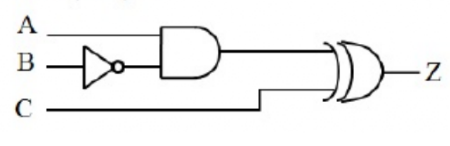
\includegraphics[width=0.4\columnwidth]{figs/q47.png}
        \caption*{}
        \label{fig:q47}
    \end{figure}
    
    \hfill{\brak{\text{GATE EC 2015}}}

    \item A 3-input majority gate is defined by the logic function $M\brak{a,b,c}=ab+bc+ca$. Which one of the following gates is represented by the function $M\brak{\overline{M\brak{a,b,c}}, M\brak{a,b,\overline{c}},c}$?
    \begin{enumerate}
    \begin{multicols}{2}
        \item 3-input NAND gate
        \item 3-input XOR gate
        \item 3-input NOR gate
        \item 3-input XNOR gate
    \end{multicols}
    \end{enumerate}
    
    \hfill{\brak{\text{GATE EC 2015}}}

    \item For the NMOSFET in the circuit shown, the threshold voltage is $V_{th}$, where $V_{th}>0$. The source voltage $V_{SS}$ is varied from 0 to $V_{DD}$. Neglecting the channel length modulation, the drain current $I_{D}$ as a function of $V_{SS}$ is represented by
    \begin{figure}[H]
        \centering
        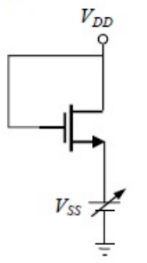
\includegraphics[width=0.3\columnwidth]{figs/q49.png}
        \caption*{}
        \label{fig:q49}
    \end{figure}
    \begin{enumerate}
        \item \begin{figure}[H]\centering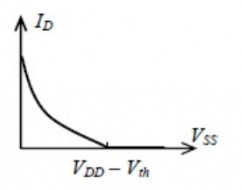
\includegraphics[width=0.4\columnwidth]{figs/q49A.png}\end{figure}
        \item \begin{figure}[H]\centering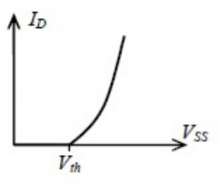
\includegraphics[width=0.4\columnwidth]{figs/q49B.png}\end{figure}
        \item \begin{figure}[H]\centering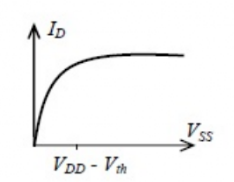
\includegraphics[width=0.4\columnwidth]{figs/q49C.png}\end{figure}
        \item \begin{figure}[H]\centering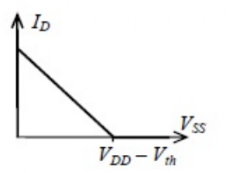
\includegraphics[width=0.4\columnwidth]{figs/q49D.png}\end{figure}
    \end{enumerate}
    
    \hfill{\brak{\text{GATE EC 2015}}}

    \item In the circuit shown, assume that the opamp is ideal. The bridge output voltage $V_{0}$ \brak{in mV} for $\delta=0.05$ is \underline{\hspace{2cm}}.
    \begin{figure}[H]
        \centering
        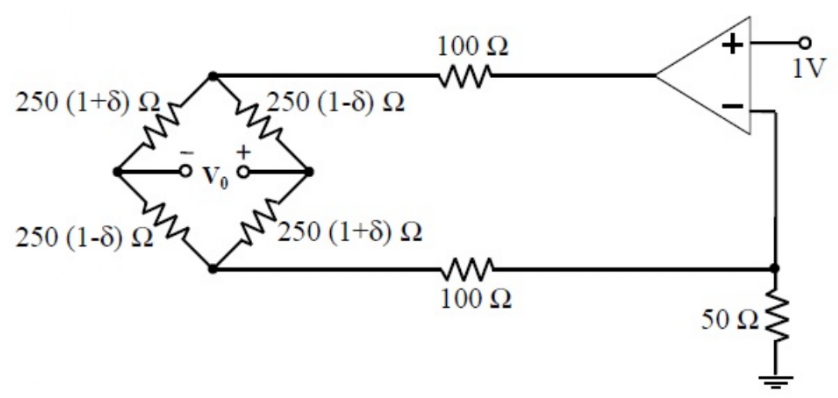
\includegraphics[width=0.7\columnwidth]{figs/q50.png}
        \caption*{}
        \label{fig:q50}
    \end{figure}
    
    \hfill{\brak{\text{GATE EC 2015}}}

    \item The circuit shown in the figure has an ideal opamp. The oscillation frequency and the condition to sustain the oscillations, respectively, are
    \begin{figure}[H]
        \centering
        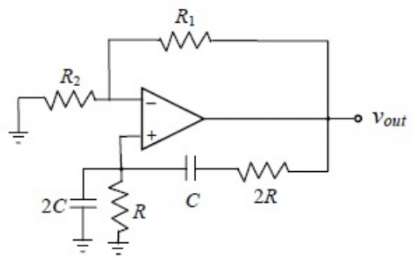
\includegraphics[width=0.5\columnwidth]{figs/q51.png}
        \caption*{}
        \label{fig:q51}
    \end{figure}
    \begin{enumerate}
        \item $\frac{1}{CR}$ and $R_{1}=R_{2}$
        \item $\frac{1}{CR}$ and $R_{1}=4R_{2}$
        \item $\frac{1}{2CR}$ and $R_{1}=R_{2}$
        \item $\frac{1}{2CR}$ and $R_{1}=4R_{2}$
    \end{enumerate}
    
    \hfill{\brak{\text{GATE EC 2015}}}

    \item In the circuit shown, $I_{1}=80$ mA and $I_{2}=4$ mA. Transistors $T_{1}$ and $T_{2}$ are identical. Assume that the thermal voltage $V_{T}$ is 26 mV at $27^{\circ}$C. At $50^{\circ}$C, the value of the voltage $V_{12}=V_{1}-V_{2}$ \brak{in mV} is \underline{\hspace{2cm}}.
    \begin{figure}[H]
        \centering
        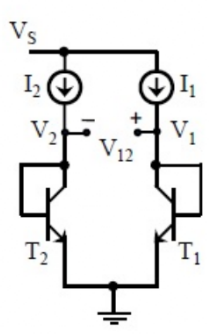
\includegraphics[width=0.3\columnwidth]{figs/q52.png}
        \caption*{}
        \label{fig:q52}
    \end{figure}
    
    \hfill{\brak{\text{GATE EC 2015}}}

    \item Two sequences $[a,b,c]$ and $[A,B,C]$ are related as,
    \[ \myvec{A\\ B\\ C} = \myvec{1 & 1 & 1\\ 1 & W_{3}^{-1} & W_{3}^{-2}\\ 1 & W_{3}^{-2} & W_{3}^{-4}} \myvec{a\\ b\\ c} \]
    where $W_{3}=e^{j\frac{2\pi}{3}}$. If another sequence $[p,q,r]$ is derived as,
    \[ \myvec{p\\ q\\ r} = \myvec{1 & 1 & 1\\ 1 & W_{3}^{1} & W_{3}^{2}\\ 1 & W_{3}^{2} & W_{3}^{4}} \myvec{1 & 0 & 0\\ 0 & W_{3}^{2} & 0\\ 0 & 0 & W_{3}^{4}} \myvec{A/3\\ B/3\\ C/3} \]
    then the relationship between the sequences $[p,q,r]$ and $[a,b,c]$ is
    \begin{enumerate}
        \item $[p,q,r]=[b,a,c]$
        \item $[p,q,r]=[b,c,a]$
        \item $[p,q,r]=[c,a,b]$
        \item $[p,q,r]=[c,b,a]$
    \end{enumerate}
    
    \hfill{\brak{\text{GATE EC 2015}}}

    \item For the discrete-time system shown in the figure, the poles of the system transfer function are located at
    \begin{figure}[H]
        \centering
        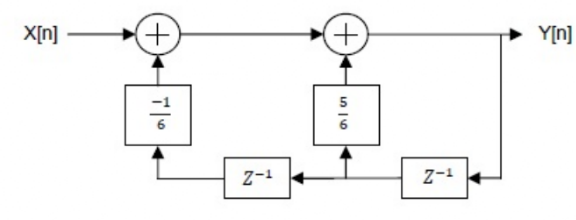
\includegraphics[width=0.6\columnwidth]{figs/q54.png}
        \caption*{}
        \label{fig:q54}
    \end{figure}
    \begin{enumerate}
        \item 2, 3
        \item $\frac{1}{2}$, 3
        \item $\frac{1}{2}$, $\frac{1}{3}$
        \item 2, $\frac{1}{3}$
    \end{enumerate}
    
    \hfill{\brak{\text{GATE EC 2015}}}

    \item The pole-zero diagram of a causal and stable discrete-time system is shown in the figure. The zero at the origin has multiplicity 4. The impulse response of the system is $h[n]$. If $h[0]=1$, we can conclude
    \begin{figure}[H]
        \centering
        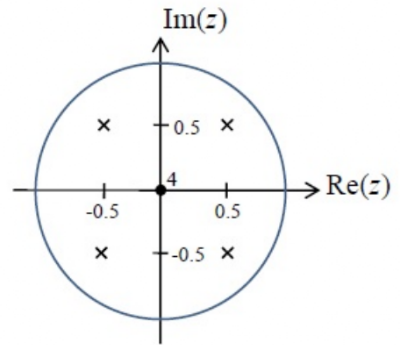
\includegraphics[width=0.4\columnwidth]{figs/q55.png}
        \caption*{}
        \label{fig:q55}
    \end{figure}
    \begin{enumerate}
        \item $h[n]$ is real for all n
        \item $h[n]$ is purely imaginary for all n
        \item $h[n]$ is real for only even n
        \item $h[n]$ is purely imaginary for only odd n
    \end{enumerate}
    
    \hfill{\brak{\text{GATE EC 2015}}}

    \item The open-loop transfer function of a plant in a unity feedback configuration is given as $G\brak{s}=\frac{K\brak{s+4}}{\brak{s+8}\brak{s^{2}-9}}$. The value of the gain $K\brak{>0}$ for which $-1+j2$ lies on the root locus is \underline{\hspace{2cm}}.
    
    \hfill{\brak{\text{GATE EC 2015}}}

    \item A lead compensator network includes a parallel combination of R and C in the feed-forward path. If the transfer function of the compensator is $G_{c}\brak{s}=\frac{s+2}{s+4}$, the value of RC is \underline{\hspace{2cm}}.
    
    \hfill{\brak{\text{GATE EC 2015}}}

    \item A plant transfer function is given as $G\brak{s}=\brak{K_{p}+\frac{K_{I}}{s}}\frac{1}{s\brak{s+2}}$. When the plant operates in a unity feedback configuration, the condition for the stability of the closed loop system is
    \begin{enumerate}
        \begin{multicols}{2}
            \item $K_{p}>\frac{K_{I}}{2}>0$
            \item $2K_{I}>K_{p}>0$
            \item $2K_{I}<K_{P}$
            \item $2K_{I}>K_{P}$
        \end{multicols}
    \end{enumerate}
    
    \hfill{\brak{\text{GATE EC 2015}}}

    \item The input X to the Binary Symmetric Channel \brak{BSC} shown in the figure is '1' with probability 0.8. The cross-over probability is $1/7$. If the received bit $Y=0$, the conditional probability that '1' was transmitted is \underline{\hspace{2cm}}.
    \begin{figure}[H]
        \centering
        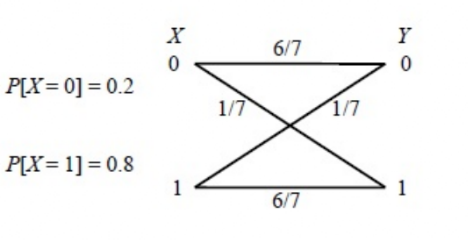
\includegraphics[width=0.4\columnwidth]{figs/q59.png}
        \caption*{}
        \label{fig:q59}
    \end{figure}
    
    \hfill{\brak{\text{GATE EC 2015}}}

    \item The transmitted signal in a GSM system is of 200 kHz bandwidth and 8 users share a common bandwidth using TDMA. If at a given time 12 users are talking in a cell, the total bandwidth of the signal received by the base station of the cell will be at least \brak{in kHz} \underline{\hspace{2cm}}.
    
    \hfill{\brak{\text{GATE EC 2015}}}

    \item In the system shown in Figure \brak{a}, $m\brak{t}$ is a low-pass signal with bandwidth W Hz. The frequency response of the band-pass filter $H\brak{f}$ is shown in Figure \brak{b}. If it is desired that the output signal $z\brak{t}=10x\brak{t}$, the maximum value of W \brak{in Hz} should be strictly less than \underline{\hspace{2cm}}.
    \begin{figure}[H]
        \centering
        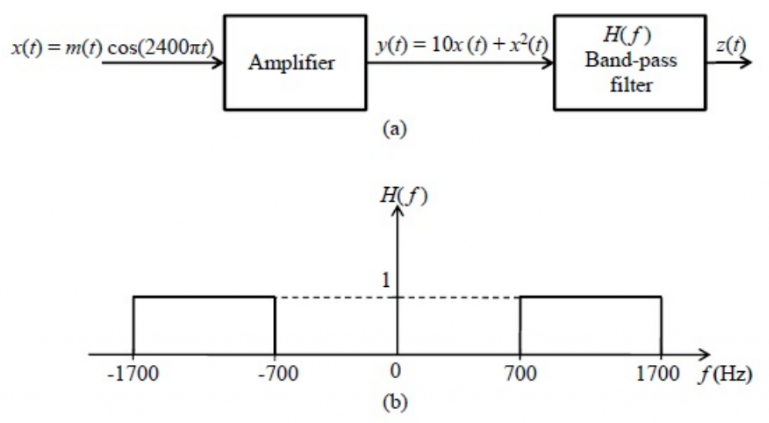
\includegraphics[width=0.8\columnwidth]{figs/q61.png}
        \caption*{}
        \label{fig:q61}
    \end{figure}
    
    \hfill{\brak{\text{GATE EC 2015}}}

    \item A source emits bit 0 with probability $\frac{1}{3}$ and bit 1 with probability $\frac{2}{3}$. The emitted bits are communicated to the receiver. The receiver decides for either 0 or 1 based on the received value R. It is given that the conditional density functions of R are as\\$f_{R|0}\brak{r}=\begin{cases}\frac{1}{4}, & -3\le r\le1,\\ 0, & otherwise,\end{cases}$ and $f_{R|1}\brak{r}=\begin{cases}\frac{1}{6}, & -1\le r\le5,\\ 0, & otherwise.\end{cases}$\\The minimum decision error probability is
    \begin{enumerate}
        \begin{multicols}{2}
            \item 0
            \item $1/12$
            \item $1/9$
            \item $1/6$
        \end{multicols}
    \end{enumerate}
    
    \hfill{\brak{\text{GATE EC 2015}}}

    \item The longitudinal component of the magnetic field inside an air-filled rectangular waveguide made of a perfect electric conductor is given by the following expression\\$H_{z}\brak{x,y,z,t}=0.1 \cos\brak{25\pi x}\cos\brak{30.3 \pi y}\cos\brak{12\pi\times10^{9}t-\beta z}\brak{A/m}$.\\The cross-sectional dimensions of the waveguide are given as $a=0.08$ m and $b=0.033$ m. The mode of propagation inside the waveguide is
    \begin{enumerate}
        \begin{multicols}{2}
            \item $TM_{12}$
            \item $TM_{21}$
            \item $TE_{21}$
            \item $TE_{12}$
        \end{multicols}
    \end{enumerate}
    
    \hfill{\brak{\text{GATE EC 2015}}}

    \item The electric field intensity of a plane wave traveling in free space is given by the following expression\\$E\brak{x,t}=a_{y}24\pi \cos\brak{\omega t-k_{0}x}\brak{V/m}$.\\In this field, consider a square area 10 cm x 10 cm on a plane $x+y=1$. The total time-averaged power \brak{\texin mW} passing through the square area is \underline{\hspace{2cm}}.
    
    \hfill{\brak{\text{GATE EC 2015}}}

    \item Consider a uniform plane wave with amplitude \brak{$E_{0}$} of 10 V/m and 1.1 GHz frequency travelling in air, and incident normally on a dielectric medium with complex relative permittivity \brak{$\epsilon_{r}$} and permeability \brak{$\mu_{r}$} as shown in the figure.
    \begin{figure}[H]
        \centering
        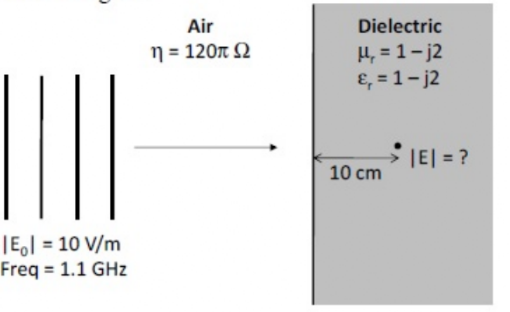
\includegraphics[width=0.7\columnwidth]{figs/q65.png}
        \caption*{}
        \label{fig:q65}
    \end{figure}
    The magnitude of the transmitted electric field component \brak{in V/m} after it has travelled a distance of 10 cm inside the dielectric region is \underline{\hspace{2cm}}.
    
    \hfill{\brak{\text{GATE EC 2015}}}

\end{enumerate}
\end{document}

